\documentclass[10pt,a4paper]{article}
\usepackage[a4paper, top=2.0cm, bottom=2.2cm, left=2.2cm, right=2.2cm, headsep=0.6cm]{geometry}
\usepackage{fontspec}
\setmainfont{texgyretermes}[Extension=.otf, UprightFont=*-regular, BoldFont=*-bold, ItalicFont=*-italic, BoldItalicFont=*-bolditalic]
\setsansfont{texgyreheros}[Extension=.otf, UprightFont=*-regular, BoldFont=*-bold, ItalicFont=*-italic, BoldItalicFont=*-bolditalic]
\usepackage{babel}
\babelprovide[import, main]{polish}
\usepackage{microtype}
\usepackage{array, booktabs, longtable, tabularx}
\usepackage[table]{xcolor}
\usepackage{graphicx}
\usepackage{enumitem}
\usepackage{parskip}
\usepackage{fancyhdr}
\usepackage{titlesec}
\usepackage[hidelinks]{hyperref}
\emergencystretch=3em
\setlist{itemsep=2pt, topsep=3pt, leftmargin=1.4em}
\definecolor{L1}{HTML}{2A78D6}\definecolor{L2}{HTML}{EB6834}\definecolor{L3}{HTML}{1BAF7A}
\definecolor{L4}{HTML}{EDA100}\definecolor{L7}{HTML}{E87BA4}\definecolor{muted}{HTML}{767A84}
\definecolor{bad}{HTML}{C23030}\definecolor{good}{HTML}{0A8A0A}
\newcommand{\linedot}[1]{\textcolor{#1}{\rule[0.1ex]{0.9ex}{0.9ex}}\,}
\newcommand{\mut}[1]{\textcolor{muted}{#1}}
\titleformat{\section}{\sffamily\large\bfseries}{\thesection.}{0.5em}{}
\titleformat{\subsection}{\sffamily\normalsize\bfseries}{\thesubsection.}{0.5em}{}
\titlespacing*{\section}{0pt}{1.2em}{0.4em}
\titlespacing*{\subsection}{0pt}{0.9em}{0.3em}
\setlength{\LTpre}{4pt}\setlength{\LTpost}{4pt}
\pagestyle{fancy}\fancyhf{}
\renewcommand{\headrulewidth}{0.3pt}
\fancyhead[L]{\sffamily\footnotesize Załącznik nr 3 do wniosku z dnia \makebox[2.4cm]{\dotfill} 2026 r.}
\fancyhead[R]{\sffamily\footnotesize Korekty rozkładu ZKM Iława}
\fancyfoot[C]{\sffamily\footnotesize \thepage}
\begin{document}
{\sffamily\footnotesize\bfseries\MakeUppercase{Załącznik nr 3 · propozycja korekt}}\par\smallskip
{\sffamily\LARGE\bfseries Korekty rozkładu ZKM Iława}\par\medskip
{\large Przesunięcia kursów o kilka minut, które dają więcej przesiadek z pociągów i do pociągów na przystanku Dworcowa.}\par\medskip
{\small\mut{Rozkład ZKM ważny od 1.09.2026. Przystanki: 005-01, 079-00. Obliczenia z dnia 29.09.2026.}}\par\bigskip
\section*{Wynik}
Obiegi autobusów, przerwy kierowców, liczba autobusów i łączny czas pracy kierowców zostają zachowane. Przesiadka jest dobra, gdy po dojściu z peronu (4 min) lub na peron (5 min) czeka się najwyżej 10 min. Liczone są pary pociąg--linia, bo podróżny potrzebuje konkretnej linii. Do przyjazdu pociągu doliczany jest zapas na typowe opóźnienie jego kategorii: EIC 3 min, EIP 3 min, IC 3 min, R 0 min, TLK 3 min. Wyniki dotyczą wariantu: obiegi jednej linii.
{\footnotesize
\begin{center}\begin{tabular}{@{}p{5.4cm} r r r@{}}\toprule
Wskaźnik & Dzień & Sobota & Niedziela \\ \midrule
Dobre przesiadki dziennie, z zapasem na opóźnienie & 148 → 244 \mut{(+65\,\%)} & 91 → 133 \mut{(+46\,\%)} & 46 → 76 \mut{(+64\,\%)} \\
Bez zapasu (pociągi punktualne) & 155 → 229 \mut{(+48\,\%)} & 91 → 124 \mut{(+36\,\%)} & 48 → 65 \mut{(+35\,\%)} \\
Rzeczywiste przyjazdy pociągów IC z minionych dni (pociąg → autobus) & 713 → 779 \mut{(+9\,\%)} & 131 → 146 \mut{(+11\,\%)} & 80 → 90 \mut{(+12\,\%)} \\
Zmienione kursy (wszystkie etapy) & 87 z 188 & 43 z 89 & 28 z 54 \\
Godziny pracy kierowców dziennie & 197,3 → 196,8 & 69,8 → 69,8 & 53,5 → 53,4 \\
Autobusy w szczycie & 18 → 18 & 6 → 6 & 5 → 5 \\
Służby z przerwą zgodną z ustawą & 34/34 → 34/34 & 11/11 → 11/11 & 10/10 → 10/10 \\
\bottomrule\end{tabular}\end{center}}
\section*{Jak czytać ten raport}
\subsection*{Słowniczek}
\begin{description}[itemsep=1pt, leftmargin=0pt]
\item[Para pociąg--linia] jeden pociąg i jedna linia ZKM. Podróżny potrzebuje konkretnej linii, więc każda para liczy się osobno.
\item[Dobra przesiadka] czekanie po dojściu najwyżej 10 min. Dojście trwa 4 min z peronu na przystanek i 5 min z przystanku na peron.
\item[Zapas na opóźnienie] do przyjazdu pociągu doliczana jest mediana opóźnienia jego kategorii: EIC 3 min, EIP 3 min, IC 3 min, R 0 min, TLK 3 min.
\item[Przesunięcie kursu] zmiana godzin kursu na wszystkich jego przystankach o tyle samo minut.
\item[Etap] grupa zmian do wprowadzenia razem: etap 1 to 20 najskuteczniejszych zmian, etap 2 to łącznie 40, ostatni etap to wszystkie. Każdy etap zachowuje zmiany poprzedniego.
\item[Zmiana towarzysząca] zmiana bez własnego zysku, potrzebna do zachowania przerwy kierowcy, postoju autobusu albo kolejności kursów po innej zmianie.
\item[Obieg] kolejne kursy jednego autobusu w ciągu dnia. Obiegi jednej linii: autobus jeździ cały dzień na tej samej linii. Obiegi mieszane: autobus może zmienić linię na Dworcowej.
\item[Postój] czas między kursami jednego autobusu.
\item[Służba] czas pracy jednego kierowcy, od przygotowania autobusu do końca ostatniego kursu.
\item[Przerwa] postój kierowcy trwający co najmniej 15 min, wliczany do przerwy wymaganej ustawą o czasie pracy kierowców.
\item[Wozokilometr, wozogodzina] kilometr i godzina pracy autobusu, razem z dojazdami z zajezdni.
\item[Wariant ostrożny, średni, optymistyczny] założenia o liczbie pasażerów: udział podróżnych kolejowych, którzy jadą dalej autobusem, i wrażliwość na czas czekania.
\end{description}
\subsection*{Metoda i założenia}
\begin{itemize}
\item \textbf{Dane.} Rozkład ZKM z rozklad.com, przetworzony do formatu GTFS. Rozkład pociągów z API PKP PLK, opóźnienia z API PKP PLK i spoznienia.me.
\item \textbf{Przesunięcia.} Kurs zmienia się najwyżej o 5 min (kursy szkolne o 2 min). Każdy zmieniony kurs i każda minuta zmiany mają karę, więc optymalizator (program całkowitoliczbowy) zmienia tylko te kursy, które coś dają.
\item \textbf{Obiegi.} Postój między kursami autobusu co najmniej 2 min. Kolejność kursów linii na Dworcowej zostaje ta sama.
\item \textbf{Koszt.} Łączny czas pracy autobusów i kierowców nie może wzrosnąć, kilometry są te same. Każda służba zachowuje przerwę wymaganą ustawą.
\item \textbf{Pociągi.} Wszystkie pociągi mają tę samą wagę.
\item \textbf{Ograniczenia.} Obiegi i służby są odtworzone z rozkładu, a nie pobrane z ZKM. Brak danych o faktycznych odjazdach autobusów. Propozycję trzeba sprawdzić z dyspozytorem ZKM przed wdrożeniem.
\item \textbf{Powtarzalność.} Narzędzie \texttt{zkmplan.py} można uruchomić po każdej zmianie rozkładu ZKM lub PKP; parametry są w pliku \texttt{zkmplan.ini}.
\end{itemize}
\section{Etapy wdrożenia}
Każdy etap zachowuje zmiany poprzedniego i dodaje kolejne, więc rozkład można zmieniać krok po kroku. Etap 1 to 20 najbardziej opłacalnych zmian, etap 2 to łącznie 40 zmian, ostatni etap nie ma limitu. Liczone z zapasem na typowe opóźnienie pociągu.
\par\medskip\noindent\begin{minipage}{\textwidth}\centering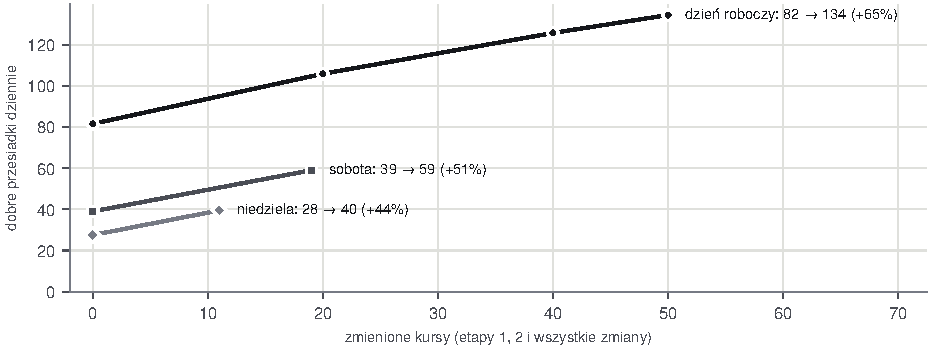
\includegraphics[width=\textwidth]{fig/korekty-etapy.pdf}\par\smallskip
{\small\mut{Rys. 1. Dobre przesiadki dziennie po kolejnych etapach.}}\end{minipage}\par\medskip
{\small
\begin{center}\begin{tabular}{@{}l l r r r@{}}\toprule
Dzień & Etap & Zmienione kursy & Dobre przesiadki/dzień & Zmiana \\ \midrule
dzień roboczy & obecny rozkład & 0 & 148 & -- \\
 & etap 1 & 20 & 180 & +22\,\% \\
 & etap 2 & 40 & 199 & +35\,\% \\
 & etap 3 & 87 & 244 & +65\,\% \\
sobota & obecny rozkład & 0 & 91 & -- \\
 & etap 1 & 20 & 117 & +29\,\% \\
 & etap 2 & 40 & 132 & +45\,\% \\
 & etap 3 & 43 & 133 & +46\,\% \\
niedziela & obecny rozkład & 0 & 46 & -- \\
 & etap 1 & 20 & 70 & +52\,\% \\
 & etap 2 & 28 & 76 & +64\,\% \\
\bottomrule\end{tabular}\end{center}}
Pełny wykaz zmienionych kursów, z pociągami, dla których przesiadka staje się dogodna, zawiera załącznik nr 1.
\section{Odjazdy z przystanku Dworcowa po korekcie}
Godziny odjazdów w dniu planowania. Zmienione godziny: obecna $\to$ \textbf{proponowana}.
\subsection*{Dzień roboczy (30.09.2026)}
{\footnotesize
\noindent\linedot{L1}1\textbf{Linia 1:} 5:05$\to$\textbf{5:07}, 6:42$\to$\textbf{6:47}, 7:24$\to$\textbf{7:26}, 8:00$\to$\textbf{8:02}, 8:35, 10:05, 11:25, 12:40, 13:08, 13:30, 14:35, 15:02$\to$\textbf{15:05}, 16:35$\to$\textbf{16:38}, 17:55, 19:55$\to$\textbf{19:52}, 21:04$\to$\textbf{21:07}\par\smallskip
\noindent\linedot{L2}2\textbf{Linia 2:} 5:38, 6:05$\to$\textbf{6:04}, 6:36, 7:00$\to$\textbf{6:56}, 7:30, 8:08$\to$\textbf{8:10}, 8:40, 9:30, 9:50, 10:23, 11:04, 11:30$\to$\textbf{11:29}, 12:10, 13:00$\to$\textbf{13:05}, 13:35$\to$\textbf{13:33}, 14:25, 14:35, 15:07, 15:30, 15:45, 16:25$\to$\textbf{16:30}, 16:50, 17:46$\to$\textbf{17:42}, 18:38, 19:08$\to$\textbf{19:10}, 19:23$\to$\textbf{19:24}, 20:06$\to$\textbf{20:02}, 20:46$\to$\textbf{20:41}, 21:06$\to$\textbf{21:07}, 22:20\par\smallskip
\noindent\linedot{L3}3\textbf{Linia 3:} 5:10, 5:52$\to$\textbf{5:54}, 6:20, 6:45, 6:52$\to$\textbf{6:54}, 7:30, 7:45, 7:52, 8:34, 9:03$\to$\textbf{9:00}, 9:41, 10:36$\to$\textbf{10:37}, 10:55$\to$\textbf{11:00}, 11:50$\to$\textbf{11:52}, 12:29, 12:36, 12:53, 13:28, 13:30, 13:38, 13:50, 14:30, 14:48, 15:16$\to$\textbf{15:14}, 15:20$\to$\textbf{15:24}, 15:40$\to$\textbf{15:42}, 16:10, 16:45, 17:15$\to$\textbf{17:14}, 18:08, 18:24, 19:27, 19:57$\to$\textbf{20:00}, 20:42$\to$\textbf{20:41}, 21:38$\to$\textbf{21:37}, 22:15\par\smallskip
\noindent\linedot{L4}4\textbf{Linia 4:} 7:30, 8:40, 9:45, 11:20$\to$\textbf{11:19}, 12:23, 13:40, 15:10\par\smallskip
\noindent\linedot{L7}7\textbf{Linia 7:} 9:15$\to$\textbf{9:14}, 15:50\par\smallskip
}
\subsection*{Sobota (3.10.2026)}
{\footnotesize
\noindent\linedot{L1}1\textbf{Linia 1:} 6:50, 8:10, 9:05$\to$\textbf{9:06}, 10:05, 11:45, 13:20$\to$\textbf{13:15}, 15:00$\to$\textbf{15:05}\par\smallskip
\noindent\linedot{L2}2\textbf{Linia 2:} 5:42$\to$\textbf{5:40}, 6:15, 6:35, 7:11$\to$\textbf{7:09}, 7:40$\to$\textbf{7:36}, 8:32, 9:25$\to$\textbf{9:24}, 10:20, 11:10, 12:01, 13:01$\to$\textbf{13:05}, 14:11, 15:10$\to$\textbf{15:08}, 16:37$\to$\textbf{16:38}, 18:10$\to$\textbf{18:09}, 20:17\par\smallskip
\noindent\linedot{L3}3\textbf{Linia 3:} 5:22$\to$\textbf{5:27}, 6:02$\to$\textbf{5:58}, 6:29, 7:04, 7:36, 7:54, 8:26$\to$\textbf{8:25}, 9:00, 9:45$\to$\textbf{9:42}, 10:35$\to$\textbf{10:33}, 10:45, 11:30, 11:52, 12:35, 13:35$\to$\textbf{13:33}, 14:05, 14:35, 15:33, 17:21$\to$\textbf{17:18}, 19:15$\to$\textbf{19:14}, 21:06$\to$\textbf{21:07}\par\smallskip
}
\subsection*{Niedziela i święta (4.10.2026)}
{\footnotesize
\noindent\linedot{L1}1\textbf{Linia 1:} 8:15$\to$\textbf{8:12}, 9:35$\to$\textbf{9:32}, 10:58$\to$\textbf{11:03}, 12:47, 14:15, 15:40$\to$\textbf{15:42}\par\smallskip
\noindent\linedot{L2}2\textbf{Linia 2:} 7:07, 9:00, 10:51$\to$\textbf{10:46}, 12:52, 14:38$\to$\textbf{14:42}, 16:32, 18:10$\to$\textbf{18:09}, 20:17\par\smallskip
\noindent\linedot{L3}3\textbf{Linia 3:} 6:05$\to$\textbf{6:04}, 7:58$\to$\textbf{8:02}, 9:16$\to$\textbf{9:14}, 10:00$\to$\textbf{10:03}, 11:00$\to$\textbf{11:03}, 11:46, 12:20$\to$\textbf{12:19}, 13:46, 14:30, 15:35$\to$\textbf{15:32}, 17:21$\to$\textbf{17:19}, 19:15$\to$\textbf{19:14}, 21:08\par\smallskip
}
\section{Obiegi autobusów i służby kierowców}
Każdy wiersz to jeden autobus, każdy pasek to kurs. Obiegi odtworzono z rozkładu, bo ZKM ich nie publikuje: autobus bierze najbliższy kurs z tego samego przystanku końcowego, najpierw tej samej linii. Przesunięcia mieszczą się w postojach, więc obiegi się nie zmieniają.
\par\medskip\noindent\begin{minipage}{\textwidth}\centering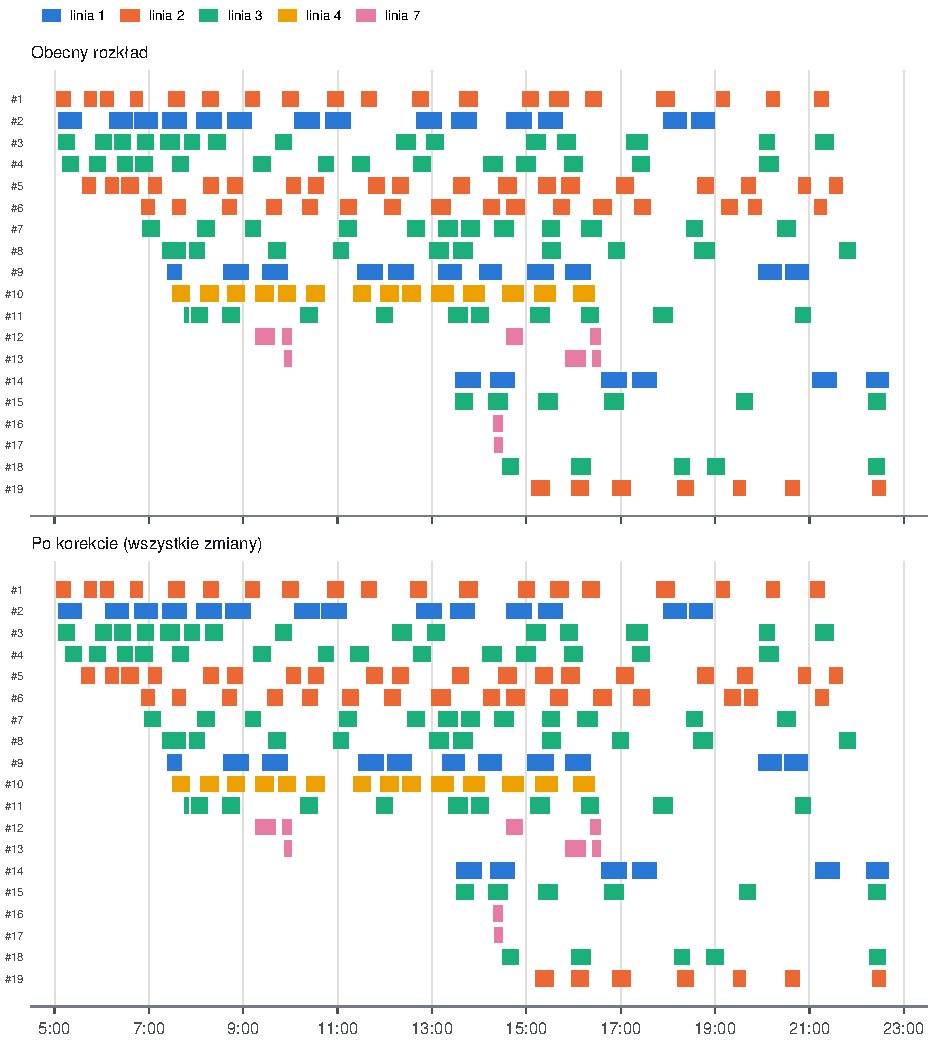
\includegraphics[width=\textwidth]{fig/korekty-obiegi.pdf}\par\smallskip
{\small\mut{Rys. 2. Obiegi autobusów w dzień roboczy (obiegi jednej linii).}}\end{minipage}\par\medskip
Obiegi podzielono na służby kierowców na Dworcowej (najdłużej 8,5 godz. z przygotowaniem). Przerwa: przy ponad 6 godz. jazdy co najmniej 30 min, przy ponad 8 godz. 45 min, w częściach po co najmniej 15 min w rozkładzie. Zgodnych służb w dzień roboczy: 34 z 34 obecnie, 34 z 34 po korekcie.
{\footnotesize
\begin{longtable}{@{}l l l r p{5.2cm} r l@{}}\toprule
Autobus & Od & Do & Jazda [h] & Przerwy [min] & Wymagane &  \\ \midrule\endhead
\bottomrule\endfoot
\#1 & 04:48 & 12:54 & 3,6 & 17, 20, 34, 22, 32, 28, 36, 21, 44 & -- & zgodna \\
\#1 & 13:18 & 21:20 & 2,8 & 53, 18, 22, 64, 56, 42, 43 & -- & zgodna \\
\#2 & 04:52 & 11:12 & 4,2 & 38, 55 & -- & zgodna \\
\#2 & 12:25 & 18:58 & 3,2 & 40, 127 & -- & zgodna \\
\#3 & 04:54 & 12:45 & 3,4 & 23, 58, 137 & -- & zgodna \\
\#3 & 12:38 & 17:38 & 1,6 & 104, 17, 66 & -- & zgodna \\
\#3 & 19:45 & 21:32 & 0,7 & 48 & -- & zgodna \\
\#4 & 04:55 & 11:40 & 2,9 & 24, 82, 61, 20 & -- & zgodna \\
\#4 & 12:21 & 20:22 & 2,4 & 65, 19, 35, 61, 140 & -- & zgodna \\
\#5 & 05:19 & 13:48 & 3,6 & 57, 57, 54, 55 & -- & zgodna \\
\#5 & 14:10 & 21:43 & 2,8 & 27, 47, 81, 30, 53, 27 & -- & zgodna \\
\#6 & 06:39 & 14:27 & 3,0 & 18, 46, 38, 27, 26, 40, 39, 36 & -- & zgodna \\
\#6 & 14:20 & 21:24 & 2,5 & 32, 37, 22, 92, 67 & -- & zgodna \\
\#7 & 06:39 & 14:48 & 3,1 & 47, 34, 102, 64, 16, 22 & -- & zgodna \\
\#7 & 15:09 & 20:48 & 1,6 & 25, 106, 100 & -- & zgodna \\
\#8 & 07:03 & 13:22 & 2,0 & 80, 65, 97 & -- & zgodna \\
\#8 & 13:13 & 18:58 & 1,6 & 92, 57, 86 & -- & zgodna \\
\#8 & 21:22 & 21:59 & 0,4 & -- & -- & zgodna \\
\#9 & 07:11 & 14:29 & 3,5 & 45, 17, 88, 30, 21 & -- & zgodna \\
\#9 & 14:50 & 21:00 & 2,1 & 15, 207 & -- & zgodna \\
\#10 & 07:15 & 14:54 & 4,9 & 16, 31, 15, 18 & -- & zgodna \\
\#10 & 14:55 & 16:28 & 0,9 & 22 & -- & zgodna \\
\#11 & 07:30 & 15:31 & 2,8 & 18, 79, 74, 70, 52 & -- & zgodna \\
\#11 & 15:55 & 21:02 & 1,1 & 69, 154 & -- & zgodna \\
\#12 & 08:59 & 16:35 & 1,2 & 269, 86 & -- & zgodna \\
\#13 & 09:37 & 16:35 & 0,8 & 343 & -- & zgodna \\
\#14 & 13:15 & 17:47 & 2,2 & 110 & -- & zgodna \\
\#14 & 20:52 & 22:45 & 1,0 & 37 & -- & zgodna \\
\#15 & 13:15 & 17:02 & 1,6 & 19, 37, 59 & -- & zgodna \\
\#15 & 19:12 & 22:38 & 0,8 & 146 & -- & zgodna \\
\#16 & 14:03 & 14:31 & 0,2 & -- & -- & zgodna \\
\#17 & 14:05 & 14:31 & 0,2 & -- & -- & zgodna \\
\#18 & 14:15 & 22:37 & 1,9 & 68, 104, 20, 183 & -- & zgodna \\
\#19 & 14:52 & 22:38 & 2,4 & 31, 26, 58, 50, 48, 92 & -- & zgodna \\
\end{longtable}}
\section{Dodatkowe kursy bez dodatkowego autobusu}
Autobusy, które czekają na Dworcowej dłużej niż jeden kurs tam i z powrotem, mogą wykonać dodatkowy kurs tej samej linii bez nowego autobusu. Gdy postój wypada w środku służby, kierowca jest już w pracy, a kurs przechodzi tylko wtedy, gdy zostaje przerwa wymagana ustawą. Gdy służba kończy się na początku postoju, kurs wydłuża ją o podany czas. Każdy kurs sprawdzono osobno.
{\footnotesize
\begin{longtable}{@{}l l l l l r r r l@{}}\toprule
Dzień & Linia & Odjazd & Powrót & Postój & Nowe dobre & Luka w linii & km & Kierowca \\ \midrule\endhead
\bottomrule\endfoot
dzień roboczy & \linedot{L3}3 & 19:14 & 21:07 & 19:12--22:15 & +5 & 63 min & 13,0 & w służbie \\
dzień roboczy & \linedot{L1}1 & 19:07 & 20:21 & 17:47--21:07 & +4 & 117 min & 20,7 & +2,6 godz. \\
dzień roboczy & \linedot{L2}2 & 17:40 & 18:58 & 17:38--19:10 & +3 & 52 min & 15,3 & w służbie \\
dzień roboczy & \linedot{L1}1 & 16:00 & 17:14 & 15:48--17:55 & +3 & 93 min & 20,7 & w służbie \\
dzień roboczy & \linedot{L1}1 & 11:14 & 12:28 & 11:12--12:40 & +3 & 80 min & 20,7 & +1,3 godz. \\
dzień roboczy & \linedot{L3}3 & 17:04 & 18:57 & 17:02--19:27 & +3 & 29 min & 13,0 & +1,9 godz. \\
dzień roboczy & \linedot{L3}3 & 17:57 & 19:50 & 17:38--20:00 & +3 & 54 min & 13,0 & +2,2 godz. \\
dzień roboczy & \linedot{L2}2 & 20:57 & 22:15 & 20:48--22:20 & +1 & 26 min & 15,3 & w służbie \\
sobota & \linedot{L3}3 & 16:48 & 17:38 & 16:25--19:14 & +5 & 105 min & 14,8 & w służbie \\
sobota & \linedot{L2}2 & 19:07 & 19:48 & 17:19--20:17 & +4 & 128 min & 15,3 & w służbie \\
sobota & \linedot{L2}2 & 16:49 & 17:30 & 15:48--18:09 & +4 & 91 min & 15,3 & w służbie \\
sobota & \linedot{L3}3 & 19:58 & 20:48 & 18:02--21:07 & +4 & 113 min & 14,8 & +2,8 godz. \\
sobota & \linedot{L2}2 & 11:05 & 11:46 & 11:03--12:01 & +3 & 50 min & 15,3 & w służbie \\
sobota & \linedot{L2}2 & 15:43 & 16:24 & 14:53--16:38 & +3 & 90 min & 15,3 & w służbie \\
sobota & \linedot{L2}2 & 10:07 & 10:48 & 10:05--11:10 & +3 & 56 min & 15,3 & w służbie \\
sobota & \linedot{L2}2 & 09:12 & 09:53 & 09:10--10:20 & +2 & 52 min & 15,3 & w służbie \\
sobota & \linedot{L2}2 & 12:12 & 12:53 & 11:54--13:05 & +2 & 64 min & 15,3 & w służbie \\
sobota & \linedot{L1}1 & 13:21 & 14:44 & 13:12--15:05 & +2 & 110 min & 20,7 & w służbie \\
sobota & \linedot{L2}2 & 08:20 & 09:01 & 08:18--09:24 & +1 & 56 min & 15,3 & w służbie \\
sobota & \linedot{L1}1 & 11:40 & 13:03 & 11:38--13:15 & +1 & 100 min & 20,7 & w służbie \\
niedziela & \linedot{L3}3 & 07:03 & 07:49 & 06:48--08:02 & +6 & 118 min & 13,0 & w służbie \\
niedziela & \linedot{L3}3 & 15:59 & 16:45 & 15:24--17:19 & +4 & 107 min & 13,0 & w służbie \\
niedziela & \linedot{L3}3 & 20:02 & 20:48 & 18:07--21:08 & +4 & 114 min & 13,0 & w służbie \\
niedziela & \linedot{L3}3 & 12:44 & 13:30 & 12:38--13:46 & +2 & 87 min & 13,0 & w służbie \\
niedziela & \linedot{L3}3 & 14:42 & 15:28 & 14:32--15:32 & +2 & 62 min & 13,0 & w służbie \\
niedziela & \linedot{L3}3 & 10:50 & 11:36 & 10:48--11:46 & +1 & 60 min & 13,0 & w służbie \\
\end{longtable}}
\section{Praca przewozowa}
Wskaźniki dzienne obecnego i proponowanego rozkładu, w obu wariantach obiegów. Wozokilometry obejmują dojazdy z zajezdni. Koszty i przychody w złotych narzędzie liczy dopiero po wpisaniu stawek i danych o sprzedaży biletów przewoźnika.
{\footnotesize
\begin{longtable}{@{}l l l r r r r r@{}}\toprule
Dzień & Obiegi & Rozkład & Autobusy & Wozokm & Wozogodz. & Służby & Godz. kierowców \\ \midrule\endhead
\bottomrule\endfoot
dzień roboczy & jednej linii & obecny & 18 & 1\,600 & 211,4 & 34 & 197,3 \\
dzień roboczy & jednej linii & proponowany & 18 & 1\,600 & 211,2 & 34 & 196,8 \\
dzień roboczy & mieszane & obecny & 15 & 1\,589 & 194,4 & 32 & 185,9 \\
dzień roboczy & mieszane & proponowany & 15 & 1\,589 & 194,3 & 32 & 185,8 \\
sobota & jednej linii & obecny & 6 & 713 & 75,6 & 11 & 69,8 \\
sobota & jednej linii & proponowany & 6 & 713 & 75,5 & 11 & 69,8 \\
sobota & mieszane & obecny & 5 & 709 & 65,1 & 10 & 59,9 \\
sobota & mieszane & proponowany & 5 & 709 & 65,1 & 10 & 59,9 \\
niedziela & jednej linii & obecny & 5 & 456 & 58,9 & 10 & 53,5 \\
niedziela & jednej linii & proponowany & 5 & 456 & 58,9 & 10 & 53,4 \\
niedziela & mieszane & obecny & 4 & 452 & 46,6 & 8 & 44,5 \\
niedziela & mieszane & proponowany & 4 & 452 & 46,6 & 8 & 44,5 \\
\end{longtable}}
\subsection*{Rok, wszystkie typy dni}
{\small
\begin{center}\begin{tabular}{@{}l l r r r r@{}}\toprule
Obiegi & Rozkład & Autobusy w szczycie & Wozokm/rok & Wozogodz./rok & Godz. kierowców/rok \\ \midrule
jednej linii & obecny & 18 & 468\,628 & 60\,925 & 56\,736 \\
jednej linii & proponowany & 18 & 468\,628 & 60\,869 & 56\,603 \\
mieszane & obecny & 15 & 465\,489 & 55\,331 & 52\,786 \\
mieszane & proponowany & 15 & 465\,489 & 55\,314 & 52\,760 \\
\bottomrule\end{tabular}\end{center}}
Jeżeli autobus może zmienić linię na Dworcowej, obecny rozkład wymaga w dzień roboczy 15 autobusów w szczycie zamiast 18, a godzin pracy kierowców jest o 6\,\% mniej. Nie wiadomo, jak ZKM układa obiegi obecnie.
\section{Ilu pasażerów mogą dać lepsze przesiadki}
Na stacji Iława Główna wsiada i wysiada średnio 4\,700 osób na dobę (Urząd Transportu Kolejowego, 2025). Część z nich przesiada się tylko między pociągami. Nie wiadomo, ilu podróżnych jedzie dalej autobusem ZKM, dlatego narzędzie liczy trzy warianty: udział autobusu i wrażliwość na czas czekania to założenia, nie pomiar. Średni czas czekania na przesiadkę (pociąg--linia, w obu kierunkach) zmienia się w dzień roboczy z 34,2 do 32,0 min ($-$6,5\,\%).
{\small
\begin{center}\begin{tabular}{@{}l r r r r r r@{}}\toprule
Wariant & Udział autobusu & Elastyczność & Przejazdy/dzień & Zmiana & Dodatkowe/dzień & Dodatkowe/rok \\ \midrule
ostrożny & 5\,\% & -0,2 & 235 & +1,3\,\% & 3 & 951 \\
średni & 10\,\% & -0,4 & 470 & +2,6\,\% & 12 & 3\,802 \\
optymistyczny & 15\,\% & -0,7 & 705 & +4,5\,\% & 32 & 9\,980 \\
\bottomrule\end{tabular}\end{center}}
\mut{\footnotesize Wartości dzienne dotyczą dnia roboczego, roczne obejmują wszystkie typy dni. Elastyczność: o tyle procent zmienia się liczba pasażerów, gdy czas czekania zmienia się o 1\,\%.}
\end{document}
